\documentclass{article}

\usepackage{geometry}
\usepackage[dutch]{babel}
\usepackage{parskip}
\usepackage{amsmath,amssymb}
\usepackage{graphicx,subcaption}

\geometry{
	paperwidth=9cm,
	paperheight=7.5cm,
	margin=0.0cm,
    paperheight=5cm
}

\begin{document}
\begin{figure}[htbp]
    \centering
    \begin{subfigure}[b]{0.45\textwidth}
        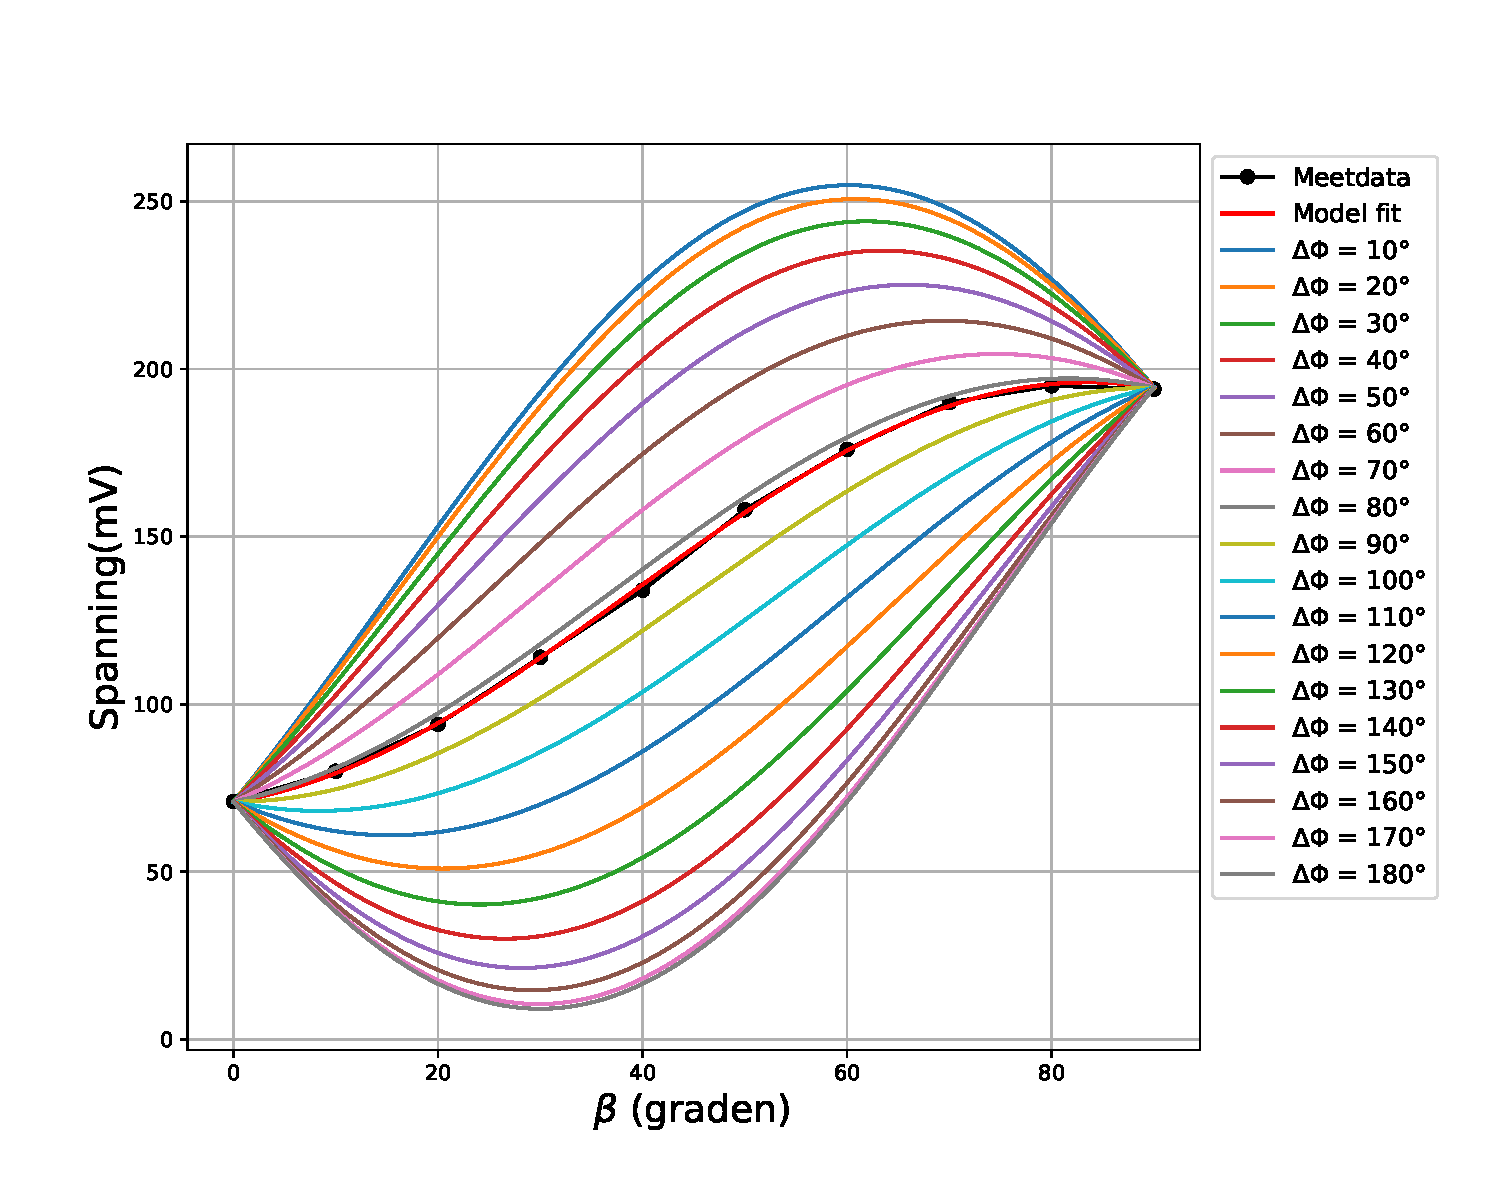
\includegraphics[width=\textwidth]{AA}
        \caption{BB}
        \label{fig:dphiExample}
    \end{subfigure}\qquad
    \begin{subfigure}[b]{0.45\textwidth}
        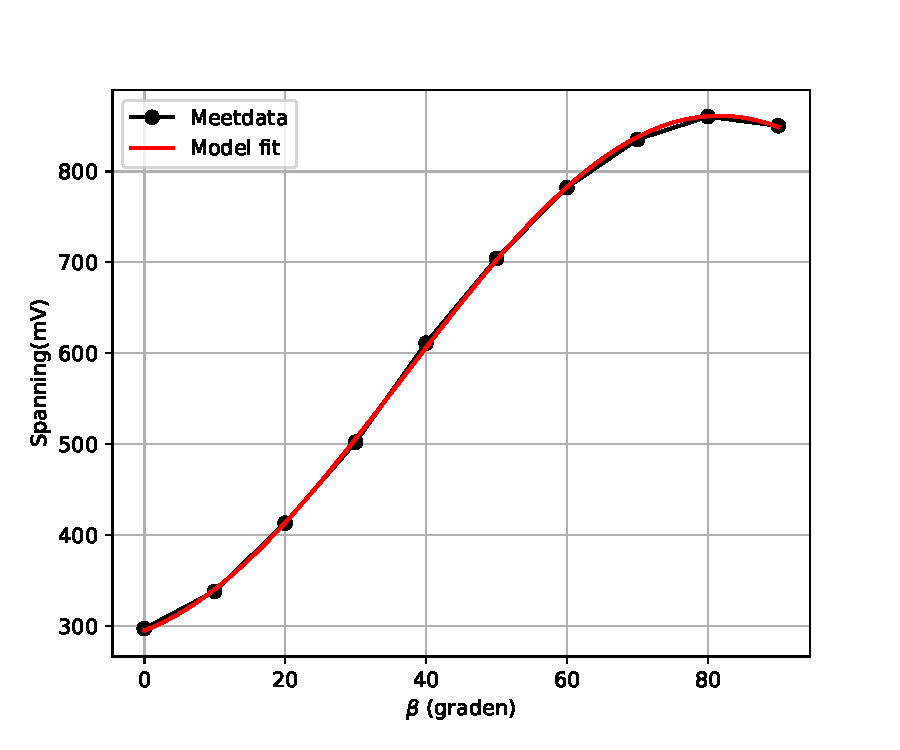
\includegraphics[width=\textwidth]{CC}
        \caption{CC}
        \label{fig:fitExample}
    \end{subfigure}
    \caption{Multiple images next to eachother!}
\end{figure}
\end{document}
